\chapter{Desarrollo de la Propuesta Solución}\label{cap:propuesta}
Este capítulo describe la arquitectura implementada, la metodología de desarrollo por fases, la estrategia de verificación y los resultados reales obtenidos al ejecutar el binario compilado. Todas las cifras provienen de los archivos \texttt{resultados/*.csv} generados por el comando \texttt{cargo run --release -- --all} con semilla 42.

\section{Metodología de desarrollo}
El proyecto siguió una metodología incremental de seis fases, en la que cada módulo debía superar sus pruebas unitarias antes de iniciar la fase siguiente:
\begin{enumerate}
\item \textbf{Álgebra lineal:} vectores, matrices y errores de dimensión.
\item \textbf{Neurona y activaciones:} Sigmoid, ReLU, lineal y sus derivadas.
\item \textbf{Pérdida:} error cuadrático medio y su gradiente.
\item \textbf{Capa y red:} propagación hacia adelante y retropropagación.
\item \textbf{Aprendizaje:} descenso de gradiente y verificación numérica de gradientes.
\item \textbf{Experimentación:} $y=2x$, XOR, vocales, prueba de escritorio y benchmarks.
\end{enumerate}

\section{Arquitectura del sistema}
El código se organiza como una biblioteca (\texttt{src/lib.rs}) y un binario de línea de comandos (\texttt{src/main.rs}). La biblioteca se divide en tres módulos con responsabilidades separadas (Tabla~\ref{tab:arquitectura}).

\begin{table}[H]
\caption{Módulos de la arquitectura implementada}\label{tab:arquitectura}
\small
\begin{tabularx}{\textwidth}{@{}l >{\raggedright\arraybackslash}X@{}}
\toprule
Archivo & Responsabilidad \\
\midrule
\texttt{math/vector.rs} & Vector $\mathbb{R}^n$: suma, resta, producto punto, Hadamard, escalamiento, norma, \texttt{argmax}. \\
\texttt{math/matrix.rs} & Matriz $\mathbb{R}^{m\times n}$ \emph{row-major}: producto matricial, matriz-vector, transpuesta, producto exterior. \\
\texttt{math/error.rs} & Tipo \texttt{MathError} para dimensiones incompatibles e índices fuera de rango. \\
\texttt{math/rng.rs} & Generador pseudoaleatorio SplitMix64 reproducible (sin crates externos). \\
\texttt{nn/activation.rs} & Trait \texttt{ActivationFn}; Sigmoid, ReLU y lineal con derivadas analíticas. \\
\texttt{nn/loss.rs} & Trait \texttt{LossFn}; MSE y su gradiente. \\
\texttt{nn/neuron.rs} & Neurona individual: pesos, sesgo, suma ponderada y activación. \\
\texttt{nn/layer.rs} & Capa densa: \texttt{forward}, \texttt{backward}, gradientes y actualización. \\
\texttt{nn/network.rs} & Red multicapa: \texttt{forward}, \texttt{backward}, \texttt{predict}, \texttt{train}, evaluación. \\
\texttt{experiments/} & Tres experimentos, prueba de escritorio, benchmarks y escritura de CSV. \\
\texttt{main.rs} & CLI reproducible: \texttt{--all}, \texttt{--exp1..3}, \texttt{--bench}, \texttt{--export}, \texttt{--seed}. \\
\bottomrule
\end{tabularx}
\par\smallskip{\footnotesize\emph{Nota.} El archivo \texttt{Cargo.toml} no declara ninguna dependencia: todo el sistema utiliza exclusivamente la biblioteca estándar de Rust.}
\end{table}

\subsection{Flujo de datos}
El flujo de una iteración de entrenamiento es: (1) la entrada $\mathbf{x}$ atraviesa cada capa calculando $\mathbf{z}^{(l)}$ y $\mathbf{a}^{(l)}$, que se almacenan en caché; (2) se calcula la pérdida MSE y su gradiente respecto a la salida; (3) cada capa, de la última a la primera, calcula $\boldsymbol{\delta}^{(l)}$, sus gradientes y el gradiente que transmite a la capa anterior; (4) todos los parámetros se actualizan con la Ecuación~\eqref{eq:gd}. El Código~\ref{cod:train} muestra que este flujo se expresa en Rust de forma casi literal.

\lstinputlisting[caption={Iteración de entrenamiento (\texttt{src/nn/network.rs})},label=cod:train]{generado/codigo/train_step.rs}

\subsection{Implementación de la retropropagación}
El Código~\ref{cod:backward} implementa las Ecuaciones~\eqref{eq:deltaL}--\eqref{eq:gradW}: el producto de Hadamard entre el gradiente recibido y la derivada de la activación produce $\boldsymbol{\delta}$; el producto exterior $\boldsymbol{\delta}\,\mathbf{x}^{\top}$ produce el gradiente de los pesos; y $\mathbf{W}^{\top}\boldsymbol{\delta}$ produce el gradiente que se transmite a la capa anterior.

\lstinputlisting[caption={Retropropagación en una capa densa (\texttt{src/nn/layer.rs})},label=cod:backward]{generado/codigo/layer_backward.rs}

\subsection{Manejo de errores de dimensión}
El Código~\ref{cod:matmul} muestra el producto matricial: antes de operar, se verifica que las dimensiones sean compatibles y, en caso contrario, se devuelve un \texttt{MathError::DimensionMismatch} que indica la operación y las formas involucradas.

\lstinputlisting[caption={Producto matricial con validación de dimensiones (\texttt{src/math/matrix.rs})},label=cod:matmul]{generado/codigo/matmul.rs}

\subsection{Reproducibilidad}
Para que cualquier evaluador obtenga exactamente los mismos resultados, los pesos iniciales y el ruido de los datos se generan con un PRNG SplitMix64 propio con semilla fija (por defecto 42), modificable mediante \texttt{--seed}.

\lstinputlisting[caption={Generador pseudoaleatorio SplitMix64 (\texttt{src/math/rng.rs})},label=cod:rng]{generado/codigo/rng.rs}

\section{Estrategia de verificación}
La suite de pruebas cuenta con 52 pruebas automatizadas (51 en la biblioteca y 1 en la CLI), todas aprobadas. Incluyen valores calculados a mano, errores de dimensión, propiedades matemáticas (por ejemplo, $(\mathbf{A}^{\top})^{\top}=\mathbf{A}$), determinismo del PRNG, convergencia real de $y=2x$ y XOR, y verificación numérica de gradientes según la Ecuación~\eqref{eq:gradcheck} sobre redes 2-4-1, 3-5-4-2 y 25-10-5. El detalle se presenta en el Anexo~\ref{anx:tests}. Adicionalmente, \texttt{cargo clippy --all-targets} no reporta advertencias.

\section{Prueba de escritorio}
La prueba de escritorio registra cada operación de las primeras iteraciones del entrenamiento. Para la neurona lineal de $y=2x$ ($\alpha = 0.01$), la primera iteración con $x=1$, $y=2$ y peso inicial $w_0 = 0.836805$, $b_0 = 0$ es:
\begin{align*}
z &= w_0 x + b_0 = 0.836805\cdot 1 + 0 = 0.836805, & a &= z = 0.836805,\\
e &= a - y = -1.163195, & \mathcal{L} &= e^2 = 1.353022,\\
\delta &= 2e\cdot f'(z) = -2.326389, & \partial\mathcal{L}/\partial w &= \delta\, x = -2.326389,\\
w_1 &= w_0 - \alpha\,\delta x = 0.860069, & b_1 &= b_0 - \alpha\,\delta = 0.023264.
\end{align*}
La Tabla~\ref{tab:escritorio} resume las diez primeras iteraciones (dos épocas). La traza completa, que también incluye las primeras iteraciones de la red XOR 2-2-1, contiene \PeFilas{} filas y se encuentra en el archivo \path{resultados/prueba_escritorio.csv}.

\begin{table}[H]
\caption{Prueba de escritorio de la neurona lineal para $y=2x$ (primeras 10 iteraciones)}\label{tab:escritorio}
\footnotesize\setlength{\tabcolsep}{3.5pt}
\begin{tabular}{@{}rrrrrrrrrr@{}}
\toprule
It. & $x$ & $y$ & $w$ & $b$ & $z$ & $e$ & $\partial\mathcal{L}/\partial w$ & $w'$ & $b'$ \\
\midrule
\TablaEscritorio
\bottomrule
\end{tabular}
\par\smallskip{\footnotesize\emph{Nota.} $e = \hat{y}-y$; $w'$ y $b'$ son los parámetros después de la actualización. Fuente: \texttt{resultados/prueba\_escritorio.csv}.}
\end{table}

\section{Experimento 1: regresión lineal $y=2x$}\label{sec:exp1}
\subsection{Diseño}
Se entrena una neurona con activación lineal (red 1-1, dos parámetros) sobre los pares $(1,2),(2,4),(3,6),(4,8),(5,10)$ durante \EunoEpocas{} épocas con $\alpha=\EunoAlpha$. La solución exacta es $w=2$, $b=0$.

\subsection{Resultados}
El MSE descendió desde \EunoMseIni{} en la época 0 hasta \EunoMseFin{} en la época \EunoEpocas. Los parámetros finales fueron $w=\EunoPesoFin$ y $b=\EunoSesgoFin$, y la predicción para el valor no visto $x=6$ fue $\hat{y}=\EunoPredSeis$ (Tabla~\ref{tab:exp1} y Figura~\ref{fig:exp1}).

\begin{table}[H]
\caption{Evolución del entrenamiento del Experimento 1}\label{tab:exp1}
\small
\begin{tabular}{@{}rrrrr@{}}
\toprule
Época & Peso $w$ & Sesgo $b$ & MSE & $\hat{y}(x=5)$ \\
\midrule
\TablaEuno
\bottomrule
\end{tabular}
\par\smallskip{\footnotesize\emph{Nota.} Fuente: \texttt{resultados/exp1\_y2x.csv}.}
\end{table}

\begin{figure}[H]
\caption{Pérdida y parámetros durante el entrenamiento de $y=2x$}\label{fig:exp1}
\centering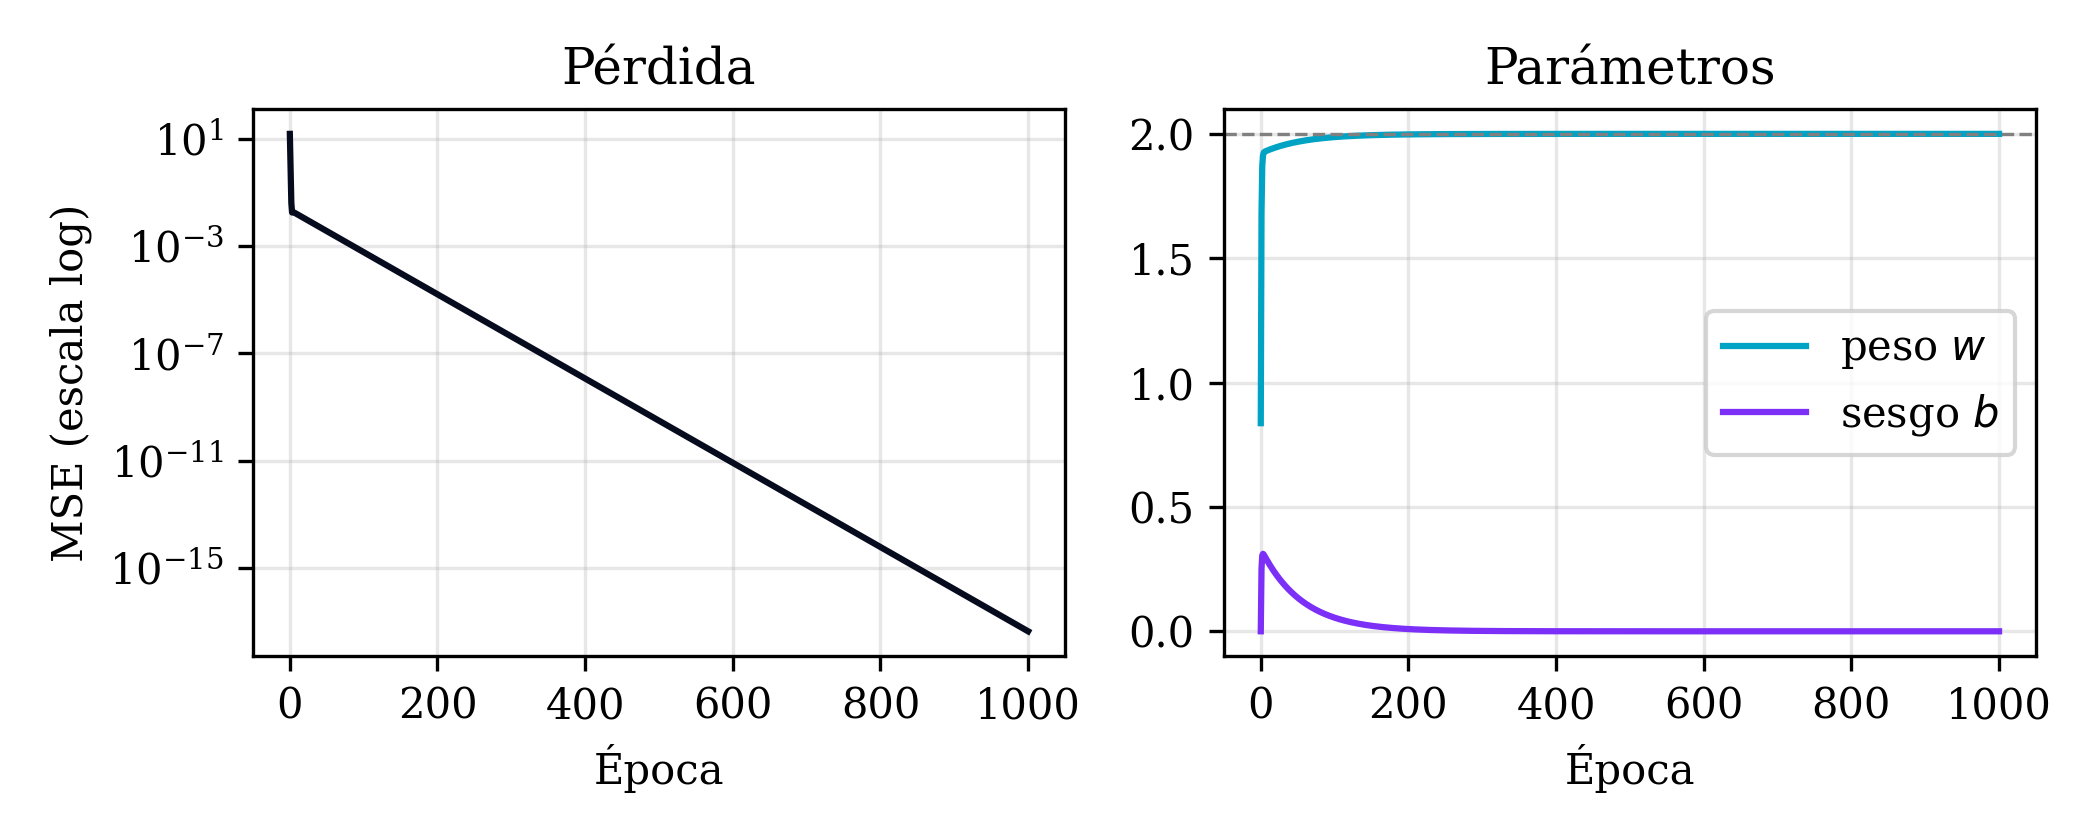
\includegraphics[width=\textwidth]{figuras/exp1_y2x.png}
\par\smallskip{\footnotesize\raggedright\emph{Nota.} Izquierda: MSE en escala logarítmica. Derecha: el peso converge a 2 (línea discontinua) y el sesgo a 0.\par}
\end{figure}

\subsection{Análisis}
La pérdida decrece de forma monótona y casi exponencial, comportamiento esperado para un problema convexo con una tasa de aprendizaje adecuada. El MSE final, del orden de $10^{-18}$, está en el límite de la precisión de la aritmética de punto flotante de doble precisión. La neurona generaliza correctamente fuera del rango de entrenamiento.

\section{Experimento 2: compuerta XOR}\label{sec:exp2}
\subsection{Diseño}
La función XOR devuelve 1 cuando sus dos entradas binarias son distintas. Se comparan un perceptrón de una capa (2-1, Sigmoid) y una red multicapa 2-4-1 (Sigmoid/Sigmoid), ambos entrenados durante \EdosEpocas{} épocas con $\alpha=\EdosAlpha$. Además, la red 2-4-1 se entrena con tres tasas: baja ($0.01$), óptima ($0.5$) y alta ($50$).

\subsection{Resultados}
El perceptrón terminó con MSE de \EdosMsePer{} y exactitud de \EdosAccPer, mientras que la red multicapa alcanzó MSE de \EdosMseMul{} y exactitud de \EdosAccMul{} (Tabla~\ref{tab:exp2}).

\begin{table}[H]
\caption{Predicciones finales para XOR}\label{tab:exp2}
\small
\begin{tabular}{@{}lrrr@{}}
\toprule
Entrada & Objetivo & Perceptrón 2-1 & Multicapa 2-4-1 \\
\midrule
\TablaEdos
\bottomrule
\end{tabular}
\par\smallskip{\footnotesize\emph{Nota.} Se clasifica como 1 cuando la salida es $\ge 0.5$. Fuente: \texttt{resultados/exp2\_xor.csv}.}
\end{table}

\begin{table}[H]
\caption{Efecto de la tasa de aprendizaje en la red 2-4-1 para XOR}\label{tab:exp2lr}
\small
\begin{tabular}{@{}lrrrl@{}}
\toprule
Escenario & $\alpha$ & MSE final & Exactitud & Época de convergencia \\
\midrule
\TablaEdosLr
\bottomrule
\end{tabular}
\par\smallskip{\footnotesize\emph{Nota.} Convergencia: primera época con MSE $<0.01$. Fuente: \texttt{resultados/exp2\_xor\_lr.csv}.}
\end{table}

\begin{figure}[H]
\caption{Curvas de pérdida del Experimento 2}\label{fig:exp2}
\centering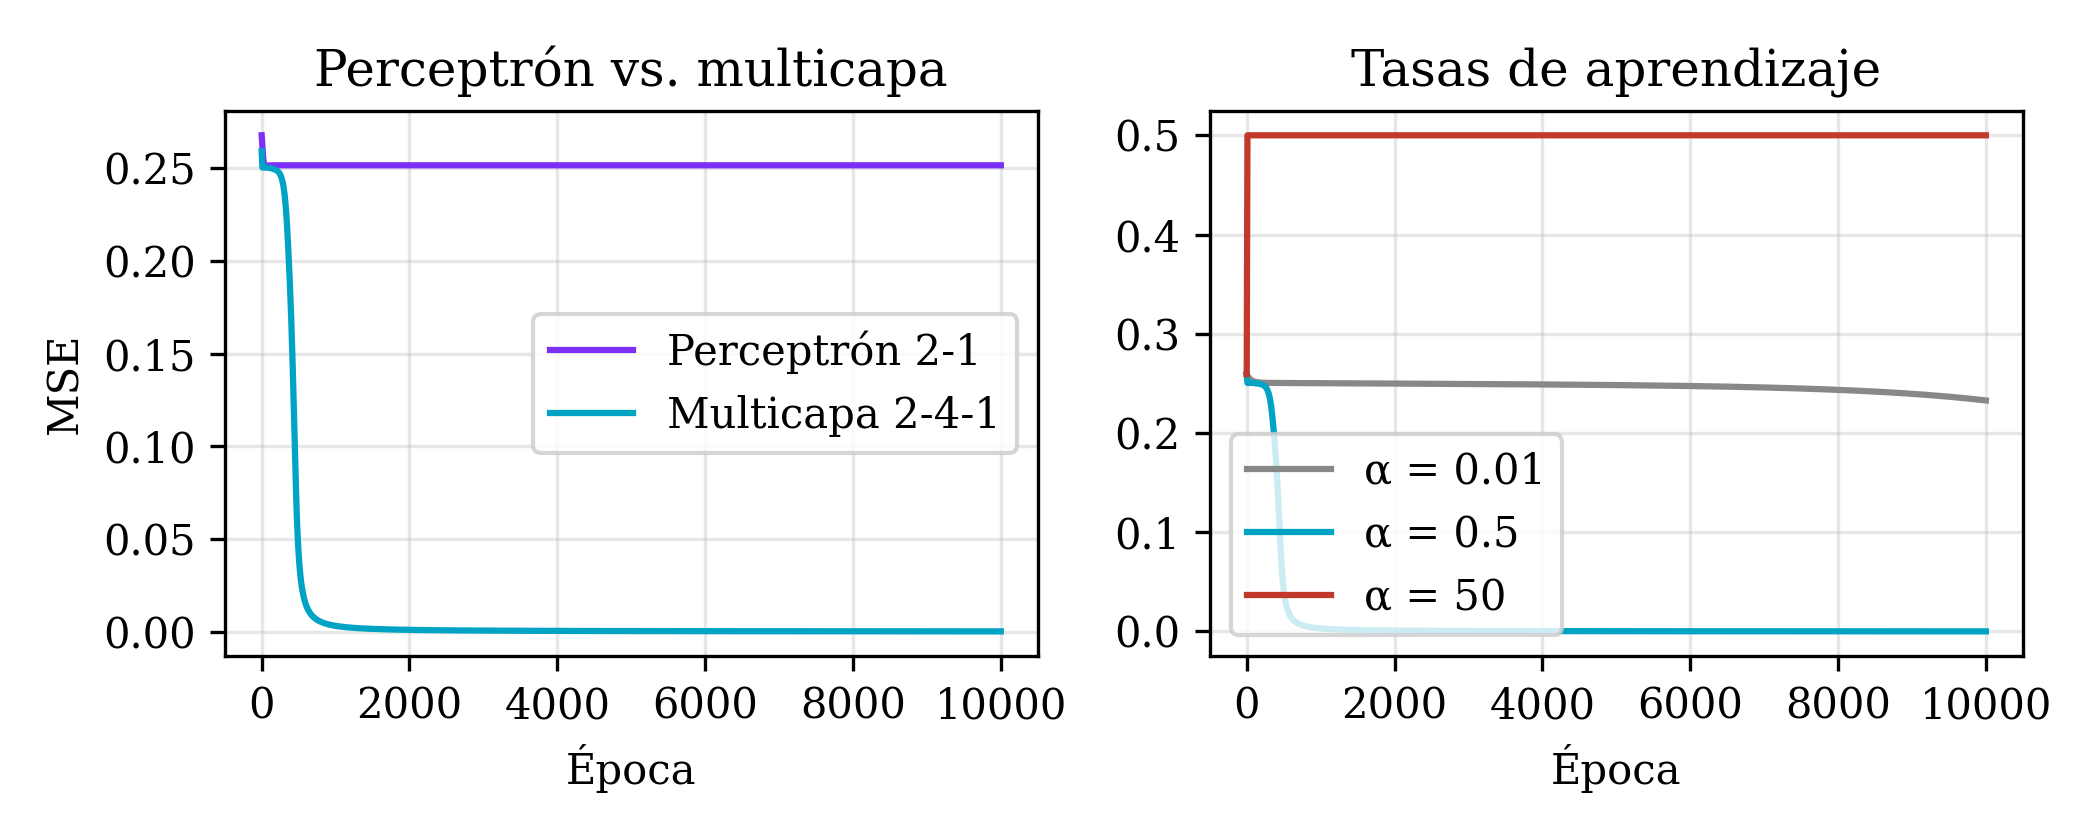
\includegraphics[width=\textwidth]{figuras/exp2_xor.png}
\par\smallskip{\footnotesize\raggedright\emph{Nota.} Izquierda: perceptrón frente a red multicapa. Derecha: tasas de aprendizaje baja, óptima y alta.\par}
\end{figure}

\subsection{Análisis}
El perceptrón no puede resolver XOR porque sus cuatro puntos no son linealmente separables: ninguna recta divide $\{(0,1),(1,0)\}$ de $\{(0,0),(1,1)\}$ \citep{minsky1969}. Su MSE se estanca cerca de $0.25$, valor que corresponde a predecir aproximadamente $0.5$ para todas las entradas. La capa oculta de la red 2-4-1 transforma el espacio de entrada en una representación donde las clases sí son separables, lo que confirma empíricamente el teorema de aproximación universal \citep{cybenko1989}.

Respecto a la tasa de aprendizaje, con $\alpha=0.01$ la red apenas avanza en \EdosEpocas{} épocas (MSE de \EdosMseBaja); con $\alpha=0.5$ converge en la época \EdosConvOptima; y con $\alpha=50$ los pasos son tan grandes que las neuronas Sigmoid se saturan, sus derivadas se anulan y el aprendizaje se detiene con MSE de \EdosMseAlta, lo que ilustra la importancia de elegir correctamente este hiperparámetro \citep{ruder2016}.

\section{Experimento 3: clasificación de vocales}\label{sec:exp3}
\subsection{Diseño del conjunto de datos}
Cada vocal se representa como una matriz binaria de $5\times5$ (Figura~\ref{fig:prototipos}), aplanada en un vector de 25 entradas. La salida usa codificación \emph{one-hot} de 5 posiciones. El conjunto de entrenamiento contiene \EtresNEnt{} muestras (los 5 prototipos y 4 variantes por vocal con un píxel invertido). El conjunto de prueba contiene \EtresNPru{} muestras distintas de las de entrenamiento: 10 variantes por vocal para cada nivel de ruido de 1 a 5 píxeles invertidos.

\begin{figure}[H]
\caption{Prototipos binarios $5\times5$ de las vocales}\label{fig:prototipos}
\centering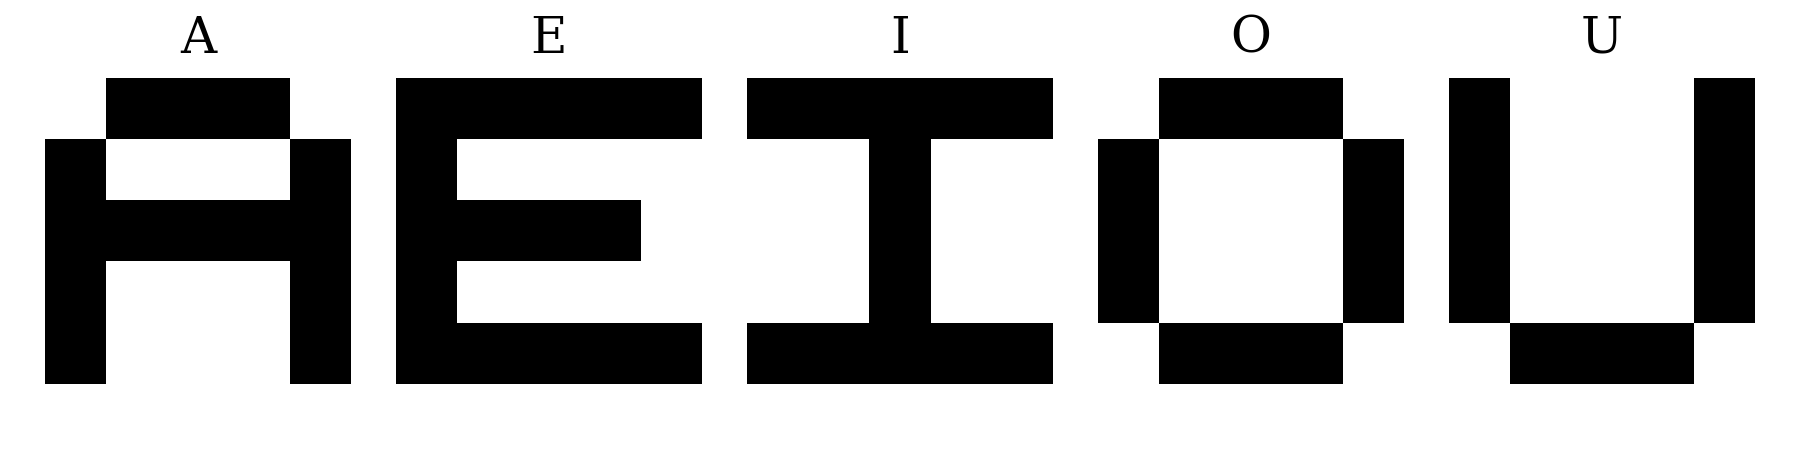
\includegraphics[width=0.75\textwidth]{figuras/vocales_prototipos.png}
\par\smallskip{\footnotesize\raggedright\emph{Nota.} Negro = 1, blanco = 0. Fuente: \texttt{resultados/dataset\_vocales.csv}.\par}
\end{figure}

\subsection{Resultados}
La red 25-10-5 (Sigmoid/Sigmoid, 315 parámetros) se entrenó durante \EtresEpocas{} épocas con $\alpha=\EtresAlpha$. Alcanzó en entrenamiento un MSE de \EtresMseEnt{} con exactitud de \EtresAccEnt, y en prueba un MSE de \EtresMsePru{} con exactitud de \EtresAccPru. La Tabla~\ref{tab:ruido} desglosa la exactitud por nivel de ruido y la Tabla~\ref{tab:confusion} presenta la matriz de confusión.

\begin{table}[H]
\caption{Exactitud de prueba por nivel de ruido}\label{tab:ruido}
\small
\begin{tabular}{@{}rrr@{}}
\toprule
Píxeles invertidos & Muestras & Exactitud \\
\midrule
\TablaEtresRuido
\bottomrule
\end{tabular}
\par\smallskip{\footnotesize\emph{Nota.} Fuente: \texttt{resultados/resumen.csv}.}
\end{table}

\begin{table}[H]
\caption{Matriz de confusión del conjunto de prueba}\label{tab:confusion}
\small
\begin{tabular}{@{}l ccccc@{}}
\toprule
& \multicolumn{5}{c}{Predicha} \\
\cmidrule(l){2-6}
Real & A & E & I & O & U \\
\midrule
\TablaConfusion
\bottomrule
\end{tabular}
\par\smallskip{\footnotesize\emph{Nota.} Filas: clase real; columnas: clase predicha. Fuente: \texttt{resultados/exp3\_confusion.csv}.}
\end{table}

\begin{figure}[H]
\caption{Entrenamiento y matriz de confusión del Experimento 3}\label{fig:exp3}
\centering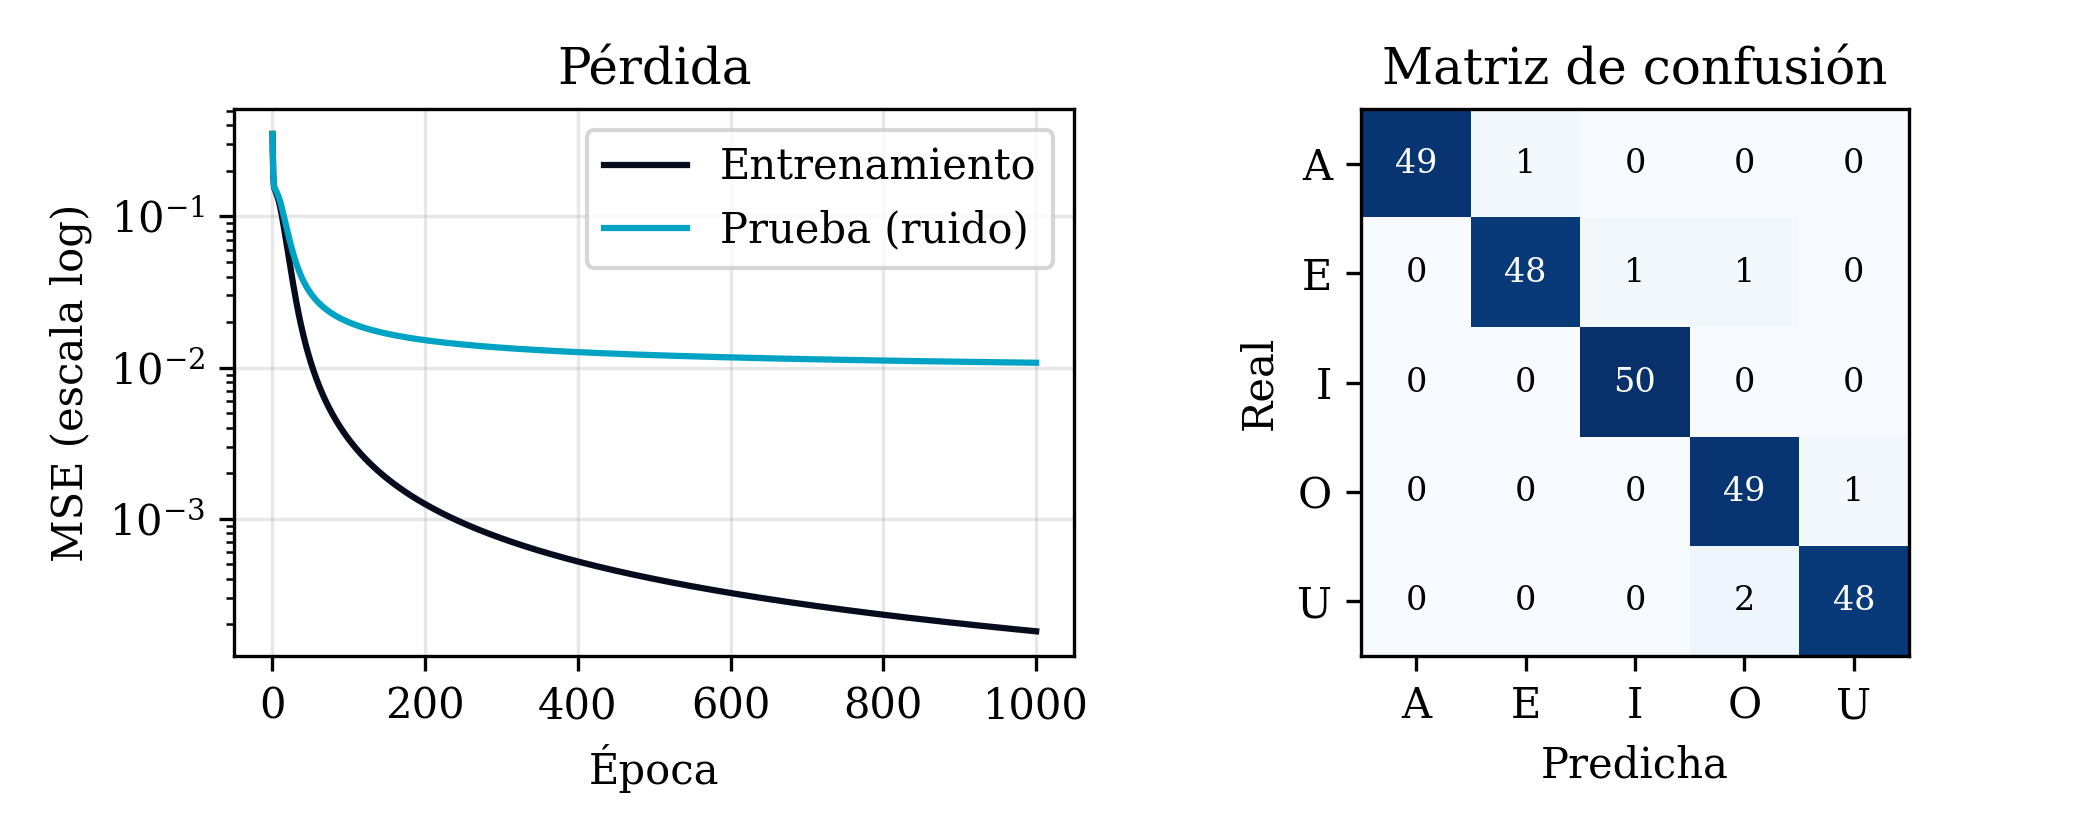
\includegraphics[width=\textwidth]{figuras/exp3_vocales.png}
\par\smallskip{\footnotesize\raggedright\emph{Nota.} Izquierda: MSE de entrenamiento y de prueba. Derecha: matriz de confusión.\par}
\end{figure}

\subsection{Análisis}
La red clasifica sin errores todas las muestras con hasta 3 píxeles invertidos (12\,\% de la imagen), aunque solo vio variantes con un píxel alterado durante el entrenamiento. Con 4 y 5 píxeles invertidos (16\,\% y 20\,\%) la exactitud desciende al 94\,\%. Los errores se concentran entre pares de vocales visualmente parecidas: O y U comparten los laterales y la base, y E comparte la columna izquierda con otras letras. Este comportamiento es coherente con la representación aprendida y muestra la capacidad de generalización del modelo frente a ruido no observado.

\section{Rendimiento y benchmarks}
Los tiempos se midieron con \texttt{std::time::Instant} sobre el binario compilado en modo \emph{release} (sistema \BenchSO, arquitectura \BenchArch), como promedio de 3 repeticiones; la inferencia se promedió sobre 100\,000 predicciones. El binario resultante ocupa \BinKiB~KiB.

\begin{table}[H]
\caption{Tiempos reales de entrenamiento e inferencia}\label{tab:bench}
\small
\begin{tabular}{@{}llrrrrr@{}}
\toprule
Experimento & Red & Parám. & Épocas & Entren. (ms) & µs/época & Inferencia (ns) \\
\midrule
\TablaBench
\bottomrule
\end{tabular}
\par\smallskip{\footnotesize\emph{Nota.} Los tiempos dependen del equipo utilizado. Fuente: \texttt{resultados/benchmarks.csv}.}
\end{table}

El costo por época se mantiene aproximadamente constante para cada arquitectura, lo que confirma la complejidad lineal $O(E\cdot N\cdot P)$ del entrenamiento (épocas $\times$ muestras $\times$ parámetros). Incluso 100\,000 épocas de XOR se completan en menos de medio segundo, lo que demuestra que no se requiere hardware especializado para estudiar estos fundamentos.
